\chapter{A Gentle Nudge Against Online Polarization}
\label{chap2}
In the previous chapter, we established the motivation for understanding complex societal phenomena through the lens of statistical physics. We now shift our focus towards a specific challenge of the digital age: the polarization of opinions in online social networks. In this chapter, we will introduce and analyze a novel intervention strategy - the ``random nudge" - that can effectively reduce polarization without causing undesirable side effects.
\section{Opinion Dynamics in Digital Social Networks}
Having examined the broader landscape of opinion formation in Chapter 1, we now focus on developing tangible solutions to the polarization challenge. As previously established, the empirically observed bimodal opinion distributions and the formation of echo chambers represent significant challenges in modern digital environments. These patterns resist the consensus predictions of traditional opinion dynamics models and create self-reinforcing information silos that impede healthy discourse.

Building on the foundation of existing models, we will adapt a recently introduced framework that successfully captures key empirical features of online opinion dynamics, including polarization, echo chambers, and the tendency for more active users to hold stronger opinions. This model provides an ideal testbed for exploring intervention strategies aimed at reducing harmful polarization.

The central question we address is whether a minimal intervention can effectively disrupt the reinforcement cycles that drive polarization without compromising individual agency or platform engagement. Specifically, we will demonstrate that a carefully calibrated "random nudge" can achieve substantial depolarization while avoiding the pitfalls of radicalization.

While Chapter 1 provided a comprehensive review of opinion dynamics models, we'll focus here on the specific framework that will enable us to test our intervention strategies. Of particular relevance is the model introduced by Baumann et al. \cite{modeling-echo-chambers-and-polarizaiton-dynamics-in-social-networks}, which successfully captures key empirical features observed in online social networks: polarized opinion distributions, echo chamber formation, and the tendency for more active users to hold more extreme opinions. This model demonstrates how homophilic interactions—the preference to connect with those holding similar opinions—naturally lead to polarized states even from initially diverse opinion distributions.

Our intervention approach is motivated by the underlying mechanism of polarization: the reinforcement of opinions through homophilic interactions. We hypothesize that by strategically disrupting this reinforcement cycle, we can achieve depolarization. Specifically, we introduce a ``random nudge" intervention that exposes agents to more diverse opinions. Through simulation and analysis, we will demonstrate that this approach can effectively break echo chambers when calibrated appropriately.

However, our findings also reveal an important caution: excessive intervention can lead to radicalization \cite{the-group-polarization-phemomenon, group-polarization-a-critical-review-and-meta-analysis}—a state where all agents adopt the same stance on an issue. This creates a delicate optimization problem: finding the precise intervention strength that reduces polarization without triggering radicalization. We will formulate and solve this optimization problem to compute the optimal nudge parameters for achieving a healthier opinion distribution.
\section{Theoretical Framework: A Model of Opinion Dynamics}
Having identified our approach, we now provide a detailed mathematical formulation of the opinion dynamics model that will serve as our experimental testbed. We adapt the framework introduced by Baumann et al. \cite{modeling-echo-chambers-and-polarizaiton-dynamics-in-social-networks}, which allows us to rigorously analyze how interventions affect the evolution of opinions in digital social networks.
\subsection{The Opinion Dynamics Framework}
The model has $N$ interacting agents, and it is assumed there are only two possible sides to an issue. This is typical of many, but not all, the issues -- for example, to allow abortion or not. Opinion on a given issue is denoted by $x_i$, which can take any real value in the range $(-\infty, \infty)$. The sign of the $x_i$ corresponds to the stance of the agent in the corresponding issue, and $|x_i|$ denotes the conviction of the agent in their respective stance. This implies that the larger the value of $|x_i|$, the more extreme the agent's opinion is. 

The model used to capture the evolution of opinion is activity driven \cite{activity-driven-modeling-of-time-varying-networks, topological-properties-of-time-integrated-activity-driven-netowork, burstiness-and-aging-in-social-temporal-networks, controlling-contagion-processes-in-activity-driven-networks}, {\it i.e.}, at each time step, only active agents are can influence other agents. Based on empirical data \cite{activity-driven-modeling-of-time-varying-networks, burstiness-and-aging-in-social-temporal-networks}, the distribution of agent's activity chosen to be,
\begin{equation}
    \label{activities.eq}
      F(a) = \frac{1-\gamma}{1-\varepsilon^{1-\gamma}} a^{-\gamma},
\end{equation}
where $a$ is the activity, $\varepsilon$ is the minimum activity (chosen in this work to be $10^{-2}$), and $\gamma$ controls how steep the function $F(a)$ which is chosen to be $2.1$. 

In simpler terms, this activity distribution means that most agents have low activity levels (they rarely post or interact), while a few agents are highly active (frequent posters) – similar to what we observe in real social media platforms where a small percentage of users generate the majority of content.

Agents' opinions evolve based on their interactions with other agents, and this information is encoded in the time-dependent adjacency matrix $A_{i, j}(t)$. Further, opinion evolution also depends on the strength of social interaction $K > 0$ and the controversialness of the issue $\alpha > 0$. The opinion dynamics is given by 
the following $N$ coupled differential equations \cite{modeling-echo-chambers-and-polarizaiton-dynamics-in-social-networks}
\begin{equation}
    \label{main.eq}
    \dot{x}_i= -x_i + K \left(\sum^{N}_{j=1} A_{ij} (t)  \tanh{(\alpha x_j)}\right).
\end{equation}
To understand this equation intuitively: an agent's opinion ($x_i$) changes based on two opposing forces – a natural tendency to moderate their view over time (the $-x_i$ term), and the influence from other agents they interact with (the sum term). The parameter $K$ determines how much weight social influence has compared to the natural moderation tendency. While people with extreme opinions have stronger influence than moderately opinionated ones, the $\tanh$ function ensures the social influence of each person is limited between $-1$ and $1$

In this, $A_{i, j}(t)$ is the temporal adjacency matrix of interaction at time $t$. If at time $t$ agent $j$ influences agent $i$, than $A_{i, j}(t) = 1$, and $A_{i, j}(t) = 0$ otherwise. If agent $i$ is active at time $t$, they will interact with $m$ other agents, weighted by the probability $P_{i, j}$. 

Further, the probabilistic reciprocity factor $r \in [0, 1]$ determines the chance that an interaction is mutually influential, {\it i.e.}, $A_{ij}(t)=A_{ji}(t)=1$. The interaction probability is defined to be a function of the magnitude between two agents' opinions.
\begin{equation}
    \label{homophily.eq}
    {P_{ij} = \frac{|x_i - x_j|^{-\beta}}{\sum_k{|x_i - x_k|^{-\beta}}}},
\end{equation}
where $\beta$ is the homophily factor which quantifies the tendency for agents with similar opinions to interact with each other: $\beta = 0$ refers to the absence of interaction preference, and $\beta > 0$ implies that the agents with similar opinions are more likely to interact with one another. Evidently, Eq.~\eqref{homophily.eq} is 
modeled as a power-law decay of connection probabilities with only a small chance for agents with opposite opinions to interact. Since most of the interactions tend to occur between agents with similar opinions, this can lead to the formation of echo chambers.

This homophily equation captures the tendency we observe in real life: people prefer to interact with those who share similar opinions. The higher the $\beta$ value, the stronger this tendency – representing how we might naturally gravitate toward content and people who reinforce our existing views, creating "filter bubbles" or echo chambers.
\subsection{The Three States of Opinion Dynamics}
\label{sec:three_states}
Now that we have established the mathematical foundation of our model, we can examine the emergent collective behaviors that arise from these individual interactions. Depending on the strength of social interaction ($K$) and the homophily factor ($\beta$), the model exhibits three distinct steady states that closely resemble opinion distributions observed in real-world scenarios.

The interaction dynamics in the model is enforced by the activity-driven temporal network that is fully encoded 
by the parameters $(\varepsilon, \gamma, m, \beta, r)$, together with the parameters that characterises the issue, $(K, \alpha)$. Asymptotically, this model features three distinct states in the distribution of opinions. If the Social interaction $K$ is sufficiently small, then the opinion of every agent decays to zero, and this state is known as the neutral consensus state. However, if social interaction $K$ is large but the homophily factor $\beta$ is small, then due to statistical fluctuations, all the opinions either become positive or negative. This state, where each agent has the same stance (the sign of $x_i$ for all $i$ is the same) with possibly different convictions, is called radicalization. It is important to note that radicalization is an absorbing state of this model. This is because when all agents have opinions with the same sign, the dynamics does not allow for a sign-change of any agent's opinion. The most interesting case emerges when social interaction $K$ and homophily factor $\beta$ are large enough. In this case, a meta-stable polarized state emerges, which is characterized by a bimodal opinion distribution.
\begin{figure}[H]
    \centering
    \includegraphics[width=\textwidth]{chapters/chapter2/consensus_radicalization_polarization.pdf}
    \caption{A schematic illustrating the three fundamental states of opinion dynamics. Panel (a): The consensus state, characterized by all agents converging to neutral opinions (near zero) in the absence of strong social interaction. Panel (b): The radicalization state, where all agents adopt the same stance (either all positive or all negative opinions) with varying degrees of conviction. Panel (c): The polarized state, featuring a bimodal opinion distribution where the population splits into two opposing groups, creating the familiar "two peaks" pattern often observed in controversial social issues.}
    \label{fig:three_states}
\end{figure}
\subsection{Quantitative Metrics for Polarization Assessmen}
\label{sec:quantifying_polarization}
Before we delve into the details of the intervention strategy and results, we discuss the three quantities employed to measure the degree of polarization based on the opinion distribution $P(x)$. They are defined as: ({\it a}) Polarization is measured through $\bar \Delta$, defined as the distance between the average of positive opinions and the average of negative opinions. {\it b}) When opinion distribution exhibits a bimodal character, the distance between the two peaks, denoted by $\Delta_{peak}$, can also be used as a measure of polarization \cite{depolarization-of-echo-chambers-by-random-dynamical-nudge}.
({\it c}) A gross measure of polarization could also be the standard deviation $\sigma$ of the entire opinion distribution \cite{link-recommendation-algorithms-and-dynamics-of-polarization-in-social-networks}. Fig.~\ref{fig:pol_def} illustrates the schematics of all three measures of polarization. It must be noted that if polarization decreases due to the intervention proposed in Eq.~\eqref{intervention.eq}, ideally, all these three quantifiers must decrease.

These measures have practical applications in analyzing real-world opinion data. For example, $\bar \Delta$ can be calculated from survey data where respondents rate their agreement with statements on a numerical scale. In social media analysis, $\Delta_{peak}$ might be observed in the distribution of sentiment scores on controversial topics, where comment sentiment often clusters around two opposing positions. The standard deviation $\sigma$ is particularly useful when analyzing large-scale data from platforms like Twitter or Reddit, where the full spectrum of opinions can be mapped and quantified.

Importantly, these metrics capture complementary aspects of polarization. $\bar \Delta$ focuses on the "distance" between opposing groups, $\Delta_{peak}$ highlights the most prominent opinion clusters, while $\sigma$ measures the overall spread regardless of modality. By tracking all three simultaneously, we can distinguish between different types of opinion shifts—for instance, distinguishing between genuine depolarization versus a shift where opinions remain far apart but become less concentrated around specific values.
\begin{figure}[H]
    \centering
    \includegraphics[width=0.8\textwidth]{chapters/chapter2/polarization_definition.pdf}
    \caption{Schematic illustration of three complementary measures of polarization used in this study. \textbf{$\bar \Delta$} (left) represents the distance between mean positive and negative opinions, capturing the average separation between opposing groups. \textbf{$\Delta_{peak}$} (center) measures the distance between the two peaks in a bimodal opinion distribution, highlighting the gap between the most common opposing viewpoints. \textbf{$\sigma$} (right) denotes the standard deviation of the entire opinion distribution, quantifying the overall spread of opinions across the population. All three metrics decrease when polarization is successfully reduced.}
    \label{fig:pol_def}
\end{figure}
\section{The Intervention: The ``Random Nudge" Strategy}
\label{sec:random_nudge}
Having established the model dynamics and identified how polarization emerges and can be measured, we now turn our attention to a key question: How can we effectively counter the formation of echo chambers and reduce polarization in online social networks?
\subsection{Mechanisms and Challenges of Echo Chamber Formation}
Echo chambers are increasingly becoming more apparent in online social media platforms. These self-reinforcing information environments arise from two primary mechanisms:
\begin{itemize}
    \item First, there is our natural tendency toward homophily—we prefer to interact with people who hold similar opinions to our own. In our model, this is captured by the homophily factor $\beta$, where larger values represent more closed and isolated echo chambers. 
    \item Second, this natural tendency is often amplified by recommendation engines on social media platforms. These algorithmically driven systems recommend similar connections or content to keep users engaged, inadvertently strengthening opinion bubbles.
\end{itemize}
The challenge lies in developing interventions that can effectively disrupt these echo chambers while simultaneously maintaining user engagement on the platforms and respecting user privacy and preferences. Such interventions should ideally not require knowledge of users' specific opinions and should create sustainable diversity rather than just temporary exposure to different viewpoints. This is a delicate balance to achieve in practice.
\subsection{The Random Nudge Mechanism}
To address these challenges, we propose a simple yet powerful intervention strategy -— the ``random nudge." The core principle is introducing a controlled amount of randomness into user interactions:

With probability $p$ (where $p < 1$), active agents will interact uniformly with any other agents in the network, regardless of opinion similarity. With the complementary probability $(1 - p)$, interactions proceed according to the normal homophily-based probability given in Eq.~\eqref{homophily.eq}.

This approach offers several advantages over more direct interventions. It preserves privacy since it requires no knowledge of agent opinions or beliefs. The intervention strength can be precisely controlled by adjusting the parameter $p$, allowing for fine-tuning based on the specific context. Additionally, it maintains the platform's engagement-driven structure while introducing just enough diversity to prevent echo chamber formation. Perhaps most importantly, it creates natural opportunities for cross-opinion exposure without forcing specific content on users, which could lead to disengagement or reactance.
\subsection{Mathematical Formulation}
We implement this random nudge by modifying the interaction probability as follows:
\begin{equation}
    \label{intervention.eq}
    \widetilde P_{ij} = p \times \frac{1}{N - 1} + (1 - p) \times P_{ij}.
\end{equation}
The first term represents the uniform random interaction (each agent has equal probability $\frac{1}{N-1}$ of interacting with any other agent), while the second term preserves the homophily-driven interactions proportional to the original $P_{ij}$. The parameter $p$ controls the strength of the intervention—higher values introduce more randomness, while values closer to zero preserve more of the natural homophily-driven structure.

This modified interaction probability is used for all subsequent simulations presented in this chapter. As we will demonstrate, even small values of $p$ can lead to dramatic reductions in polarization and the breakdown of echo chambers.
\section{Empirical Results of the Random Nudge Intervention}
\label{sec:results}
With the intervention strategy introduced in Sec.~\ref{sec:random_nudge}, we find that with sufficiently small random nudge probability $p$, significant depolarization can be obtained, which is evident as the opinion distributions approach towards a unimodal distribution along with the decay of all three measures of polarization. To see the effects of nudge, we perform numerical simulations of the basic model in Eq.~\eqref{main.eq} using the interaction probability given in Eq.~\eqref{homophily.eq} and the intervention model in Eq.~\eqref{intervention.eq}. The simulations are performed with $N=5000$ agents for $1000$ time steps with $dt=0.01$. At initial time $x_i$ is uniformly chosen from a small interval, {\it i.e.}, $x_i \in [-1,1]$ for $i=1,2 \dots N$. The model parameters are chosen to be $\alpha=3$, $\beta=3$, $K=3$, $m=10$, $\gamma=2.1$, $\varepsilon=0.01$ and $r=0.5$ for all the simulations unless mentioned otherwise. The parameters chosen for the simulations lead to a polarized state in the original model without intervention. Our analysis reveals several key insights into how small perturbations can lead to significant changes in collective behavior patterns.
\subsection{Depolarization Effects}
In Fig.~\ref{fig:trajectory}, we show the contrast between the trajectories of individual opinions and the opinion distribution with and without the application of a nudge. In the absence of nudge ($p=0$), the simulation results in Fig.~\ref{fig:trajectory}(a) show fewer trajectories with opinions $x_i \approx 0$. This leads to a bimodal distribution of opinions characteristic of a polarized state. In contrast, in Fig.~\ref{fig:trajectory}(b), a small nudge with a probability of $p = 0.01$ is applied, and we find significantly more trajectories with moderate opinions. This, effectively, is seen to lead to an absence of polarization, which is evident from the unimodal opinion distribution. The magnifications of the region around $x_i=0$ and its distribution (shown in Fig.~\ref{fig:trajectory}) reveal a clear distinction between these two scenarios.
\begin{figure}[H]
    \centering
    \includegraphics[width=\textwidth]{chapters/chapter2/polarized_and_depolarized_trajectories.pdf}
    \caption{Visualization of opinion trajectories and resulting distributions with and without the random nudge intervention. (a) Without nudge ($p=0$): Opinion trajectories show clear divergence, avoiding the moderate region around $x=0$ (shown in the magnification). The resulting distribution (right panel) is distinctly bimodal, indicating strong polarization with few moderate opinions. (b) With a small nudge ($p=0.01$): Opinion trajectories show significant crowding around $x=0$ (magnification), leading to a nearly unimodal symmetric distribution (right panel). This demonstrates how even a minimal random intervention can substantially reduce polarization by promoting moderate viewpoints.}
    \label{fig:trajectory}
\end{figure}
\subsection{Network Effect: Breaking of Distinct Clusters}
To examine the effect of network nudge, we analyze the underlying time-averaged structures of the temporal interactions network. Without nudge, the interaction network has two distinct clusters; most of the connections are among positive opinionated agents or negative opinionated agents. There exist very few connections between these two groups other than for the agents with extreme opinions.
This is expected since the agents with extreme opinions are also those who tend to be more active on social networks fora; hence on average, they form more connections. This enables them to be relatively more connected to the agents with opposing opinions. These results are visually depicted in Fig.~\ref{fig:network} as two snapshots of evolving network diagrams. If $p=0$, no nudge is applied. In this case, as Fig.~\ref{fig:network}(b) shows, a polarized network, made up of two distinct blue and red-colored clusters, is formed. Blue color corresponds to nodes with $x > 0$, and red color to $x< 0$. The opinion distribution shown in Fig.~\ref{fig:network}(a) confirms the existence of polarization.

However, when a nudge is applied, even for the case when the nudge probability is as small as $p = 0.01$, we find the network to be well mixed (large blue and red clusters have disappeared) (Fig.~\ref{fig:network}(e)), and this leads to a significantly depolarized state indicated by the approximate unimodality of the opinion distribution as shown in Fig.~\ref{fig:network}(d).
\begin{figure}[H]
    \centering
    \includegraphics[width=\textwidth]{chapters/chapter2/echochamber.jpg}
    \caption{Comprehensive analysis showing how random nudges affect opinion distribution, network structure, and echo chamber formation. Top row (a-c): No nudge ($p=0$) condition showing (a) polarized opinion distribution, (b) segregated network with two distinct clusters (blue nodes for positive opinions, red for negative, with color saturation indicating conviction strength), and (c) two distinct lobes in the heatmap of agent opinions versus their neighbors' mean opinions, confirming strong echo chamber effects. Bottom row (d-f): With nudge ($p=0.01$) showing (d) depolarized, single-peak opinion distribution, (e) well-mixed network without clear clustering, and (f) single-lobed heatmap confirming the successful weakening of echo chambers. This demonstrates how a small intervention in connection patterns can fundamentally alter the macro-level opinion landscape.}
    \label{fig:network}
\end{figure}
The term echo chamber describes a situation where the beliefs or opinions of people are reinforced by interactions among a closed group of people who hold similar opinions. In recent years, this has been widely discussed in the context of online communities \cite{echo-chambers-emotional-contagion-and-group-polarization-on-facebook, quantifying-echo-chamber-effects-in-information-spreading-over-political-communication, political-discourse-on-social-media-echo-chambers, The-echo-chamber–effect-on-social-media}. However, some studies appear to suggest that the effects of echo chambers are over-estimated \cite{the-echo-chamber-is-overstated}. To infer the presence of echo chamber-type effects, we calculate the average opinion of the nearest neighbors (NN) of each agent \cite{modeling-echo-chambers-and-polarizaiton-dynamics-in-social-networks, The-echo-chamber–effect-on-social-media}. This is denoted by 
\begin{equation}
\langle x_{NN}\rangle = k_i^{-1} \sum_j {a_{ij} x_j}, ~~~\mbox{and}~~~ k_i = \sum_j{a_{ij}},
\label{eq.xnn}
\end{equation}
where $a_{ij}$ is the temporally aggregated (over the last 100 time-steps) adjacency matrix. When a nudge is not applied ($p=0$), a colored heatmap of $x$ and $\langle x_{NN}\rangle$, in Fig.~\ref{fig:network}(c) reveals two disjoint hot spots corresponding to the two distinct echo chambers. And we find a strong bimodality in the marginal distributions.
Now, when we apply a nudge with probability $p=0.01$, we can observe only one hot spot indicating the existence of only one closed group (Fig.~\ref{fig:network}(f)). All the agents are inside this closed group, and the echo chamber effect is largely diluted or non-existent. We did not find perfect unimodality in the marginal distribution of $x$, which can be attributed to the fact that different realizations can lead to either of these three distributions: (a) slight bimodal distribution with signification reduction in all three polarization parameters, (b) unimodal distribution with a slight skew towards positive opinions and (c) similar distribution with a skew towards negative opinions. As the heat maps and the marginal distributions are created from data averaged over 200 realizations, all the above factors contribute to the slight bimodality in the marginal distribution of $x$. Nevertheless, the marginal distribution corresponds to a signification reduction in polarization and echo chambers.
\subsection{Quantitative Analysis of Polarization Reduction}
To obtain a global picture of how depolarization sets in as a function of nudge probability $p$, we plot the three measures of polarization as a function of $p$. All three measures, $\bar\Delta, \Delta_{peak}$ and $\sigma$, have been computed from the simulation results. The results shown represent an average over the last 100 time steps of the simulations and averaged over 200 realizations. In Fig.~\ref{fig:pol_par}, we observe that all three measures of polarization decrease as the strength of the nudge $p$ increases. In particular, $\bar \Delta$ and $\sigma$ are found to decrease as a stretched exponential function $\exp(-p^\gamma)$, and the stretching factor $\gamma$ is determined through regression to be approximately $0.3$. A recent work studying the depolarization of echo chambers \cite{depolarization-of-echo-chambers-by-random-dynamical-nudge} considered adding an effective noise term dependent on a random sample of opinions to Eq.~\eqref{main.eq}. While this approach succeeds in making the opinion distribution unimodal, it increases the width of the distribution significantly, which as a consequence, corresponds to an increase in extreme opinions. To quantify the effect of the nudge on the extreme opinions, we define $f_{ext}$ as the fraction of agents with conviction $|x| > x_{th}$, where $x_{th}$ is a positive threshold. And indeed our framework of nudging the mechanism of forming social connections in online interactions works well in decreasing width of the opinion distribution (Fig.~\ref{fig:pol_par} (c)) as well as extreme opinions Fig.~\ref{fig:pol_par} (d) and also suggests direct algorithmic interventions for recommender systems.

In the original model, the authors found the polarized state to be meta-stable and showed that with an increased value of $\beta$, the lifetime of the state has a faster than exponential growth. Our intervention adds more randomness to the system and increases statistical fluctuations. Hence for large $p$, we observe a drastic decrease in the average lifetime of the polarized and depolarized states. An approximate straight line in the log-log plot indicates the lifetime of polarized or depolarized states decreases as a power law as nudge strength $(p)$ is increased (see Fig.~\ref{fig:pol_par} (e)). Fig.~\ref{fig:pol_par} (f) also captures the same effect as we see that radicalization is either non-existent or a rarity for $p < 10^{-2}$, but it increases quickly and becomes a norm for $p > 10^{-2}$.
\begin{figure}[H]
    \centering
    \includegraphics[width=\textwidth]{chapters/chapter2/parameters_vs_nudge.pdf}
    \caption{Quantitative analysis of polarization measures as functions of nudge strength $p$. (a-c) Three measures of polarization: (a) $\bar\Delta$ (distance between mean opinions), (b) $\Delta_{peak}$ (distance between peaks), and (c) $\sigma$ (standard deviation of opinions) all decrease with increasing nudge strength, following an approximate stretched exponential decay. (d) The fraction of agents with extreme opinions ($f_{ext}$) similarly decreases, showing the nudge reduces extremism alongside polarization. (e) The lifetime of polarized states decreases as a power law with increasing nudge strength, indicating faster transitions to radicalization state. (f) The fraction of simulations resulting in radicalization increases sharply beyond $p \approx 10^{-2}$, revealing the critical threshold where the intervention begins producing undesirable outcomes. All results represent averages over 200 simulations, excluding radicalized cases for panels (a-d).}
    \label{fig:pol_par}
\end{figure}
\section{Balancing Depolarization Against Radicalization Risk}
In many situations, radicalization is as much undesirable as polarization. Hence to solve the issue of radicalization at a high value of nudge probability, rather than nudging all the people in the population, at each time step of the simulation, we randomly select $f$ fraction of the population and nudged them. We define a simple linear utility function $U(\bar \Delta, f_{rad}) = \tilde{\bar \Delta} + f_{rad}$
Where $\tilde{\bar \Delta}$ is $\bar \Delta$, linearly scaled to be between $0$ and $1$, and $f_{rad}$ is the fraction of radicalized
simulations. The structure of the utility function is the same for the other two measures of polarization.
\subsection{Finding the Sweet Spot: Optimizing the Nudge}
This utility function represents a fundamental trade-off: we want to minimize both polarization (measured by $\bar{\Delta}$) and the risk of radicalization ($f_{rad}$). In practical terms, this means finding intervention parameters that create enough opinion diversity to prevent echo chambers, but not so much randomness that the system tips into a radicalized state.

Fig.~\ref{fig:optimization} depicts the heat map of the utility functions corresponding to the three utility functions. The optimal population fraction and nudge probability is numerically found to follow the curve $p\cdot f^A = B$, where $A$ and $B$ are constants.
\begin{figure}[H]
    \centering
    \includegraphics[width=\textwidth]{chapters/chapter2/optimization_heatmap.pdf}
    \caption{Optimization analysis for balancing depolarization against radicalization risk. The heatmaps show utility values (combining polarization reduction and radicalization avoidance) as functions of nudge strength $p$ and population fraction $f$ being nudged. Panels (a), (b), and (c) correspond to utilities based on $\bar \Delta$, $\Delta_{peak}$, and $\sigma$ measures respectively. The red dashed curves, following $p\cdot f^A = B$ (where $A$ and $B$ are constants), indicate the optimal parameter combinations that maximize depolarization while minimizing radicalization risk. This analysis provides practical guidance for implementing nudge strategies in real-world systems by showing that nudging a smaller fraction of the population more strongly can be as effective as nudging everyone weakly.}
    \label{fig:optimization}
\end{figure}
This power-law relationship reveals an important insight: there's a mathematical trade-off between how many people we nudge ($f$) and how strongly we nudge them ($p$). For example, it suggests that nudging 10\% of the population with a stronger intervention might be as effective as nudging everyone with a weaker intervention. This finding has significant practical implications for platform design, as it means targeted interventions could potentially be as effective as system-wide changes while requiring less disruption to the overall user experience.
\section{Robustness Check: Testing on Alternative Models}
To ensure the robustness of our intervention framework, we applied network nudge to another recent model \cite{modeling-explosive-opinion-depolarization-in-interdependent-topics} of opinion dynamics, which, together with homophily, exhibits the effect of echo chambers. This validation demonstrates that the random nudge strategy is not limited to a single model but represents a more general principle for disrupting echo chambers across different mathematical frameworks. The dynamics of the model is governed by the following $N$ coupled differential equations:
\begin{equation}
    \label{new_model.eq}
    \dot{x}_i(t)= |x_i|\sin{(x_i^0- x_i)} + K \left(\sum^{N}_{j=1} A_{ij} (t)  \sin{(x_i - x_j)}\right).
\end{equation}
In contrast to the original model \cite{modeling-explosive-opinion-depolarization-in-interdependent-topics}, the variable $x_i$ is chosen to be the opinions of the people on a single topic, and the temporal adjacency matrix is formed according to homophily probability~\eqref{homophily.eq}. $x_i^0$ is the initial opinion of agent $i$, and all the other variables and parameters have the same meaning as in the previous model~\eqref{main.eq}. In Fig.~\ref{fig:new_model}, we show that When the social interaction and the homophily factor are high enough ($K = 4$, $\beta = 4$), many echo chambers are formed, which is clear from the trajectories of the opinion as well as from the multiple communities seen in the aggregated network (Fig.~\ref{fig:new_model} (a, b)). But when we introduce a slight nudge ($p = 0.002$), The effect of echo chambers is reduced drastically. The opinion trajectories seem to converge to a moderate value, and the interaction network is well-connected without any obvious segregated communities (Fig.~\ref{fig:new_model} (c, d)).
\begin{figure}[H]
    \centering
    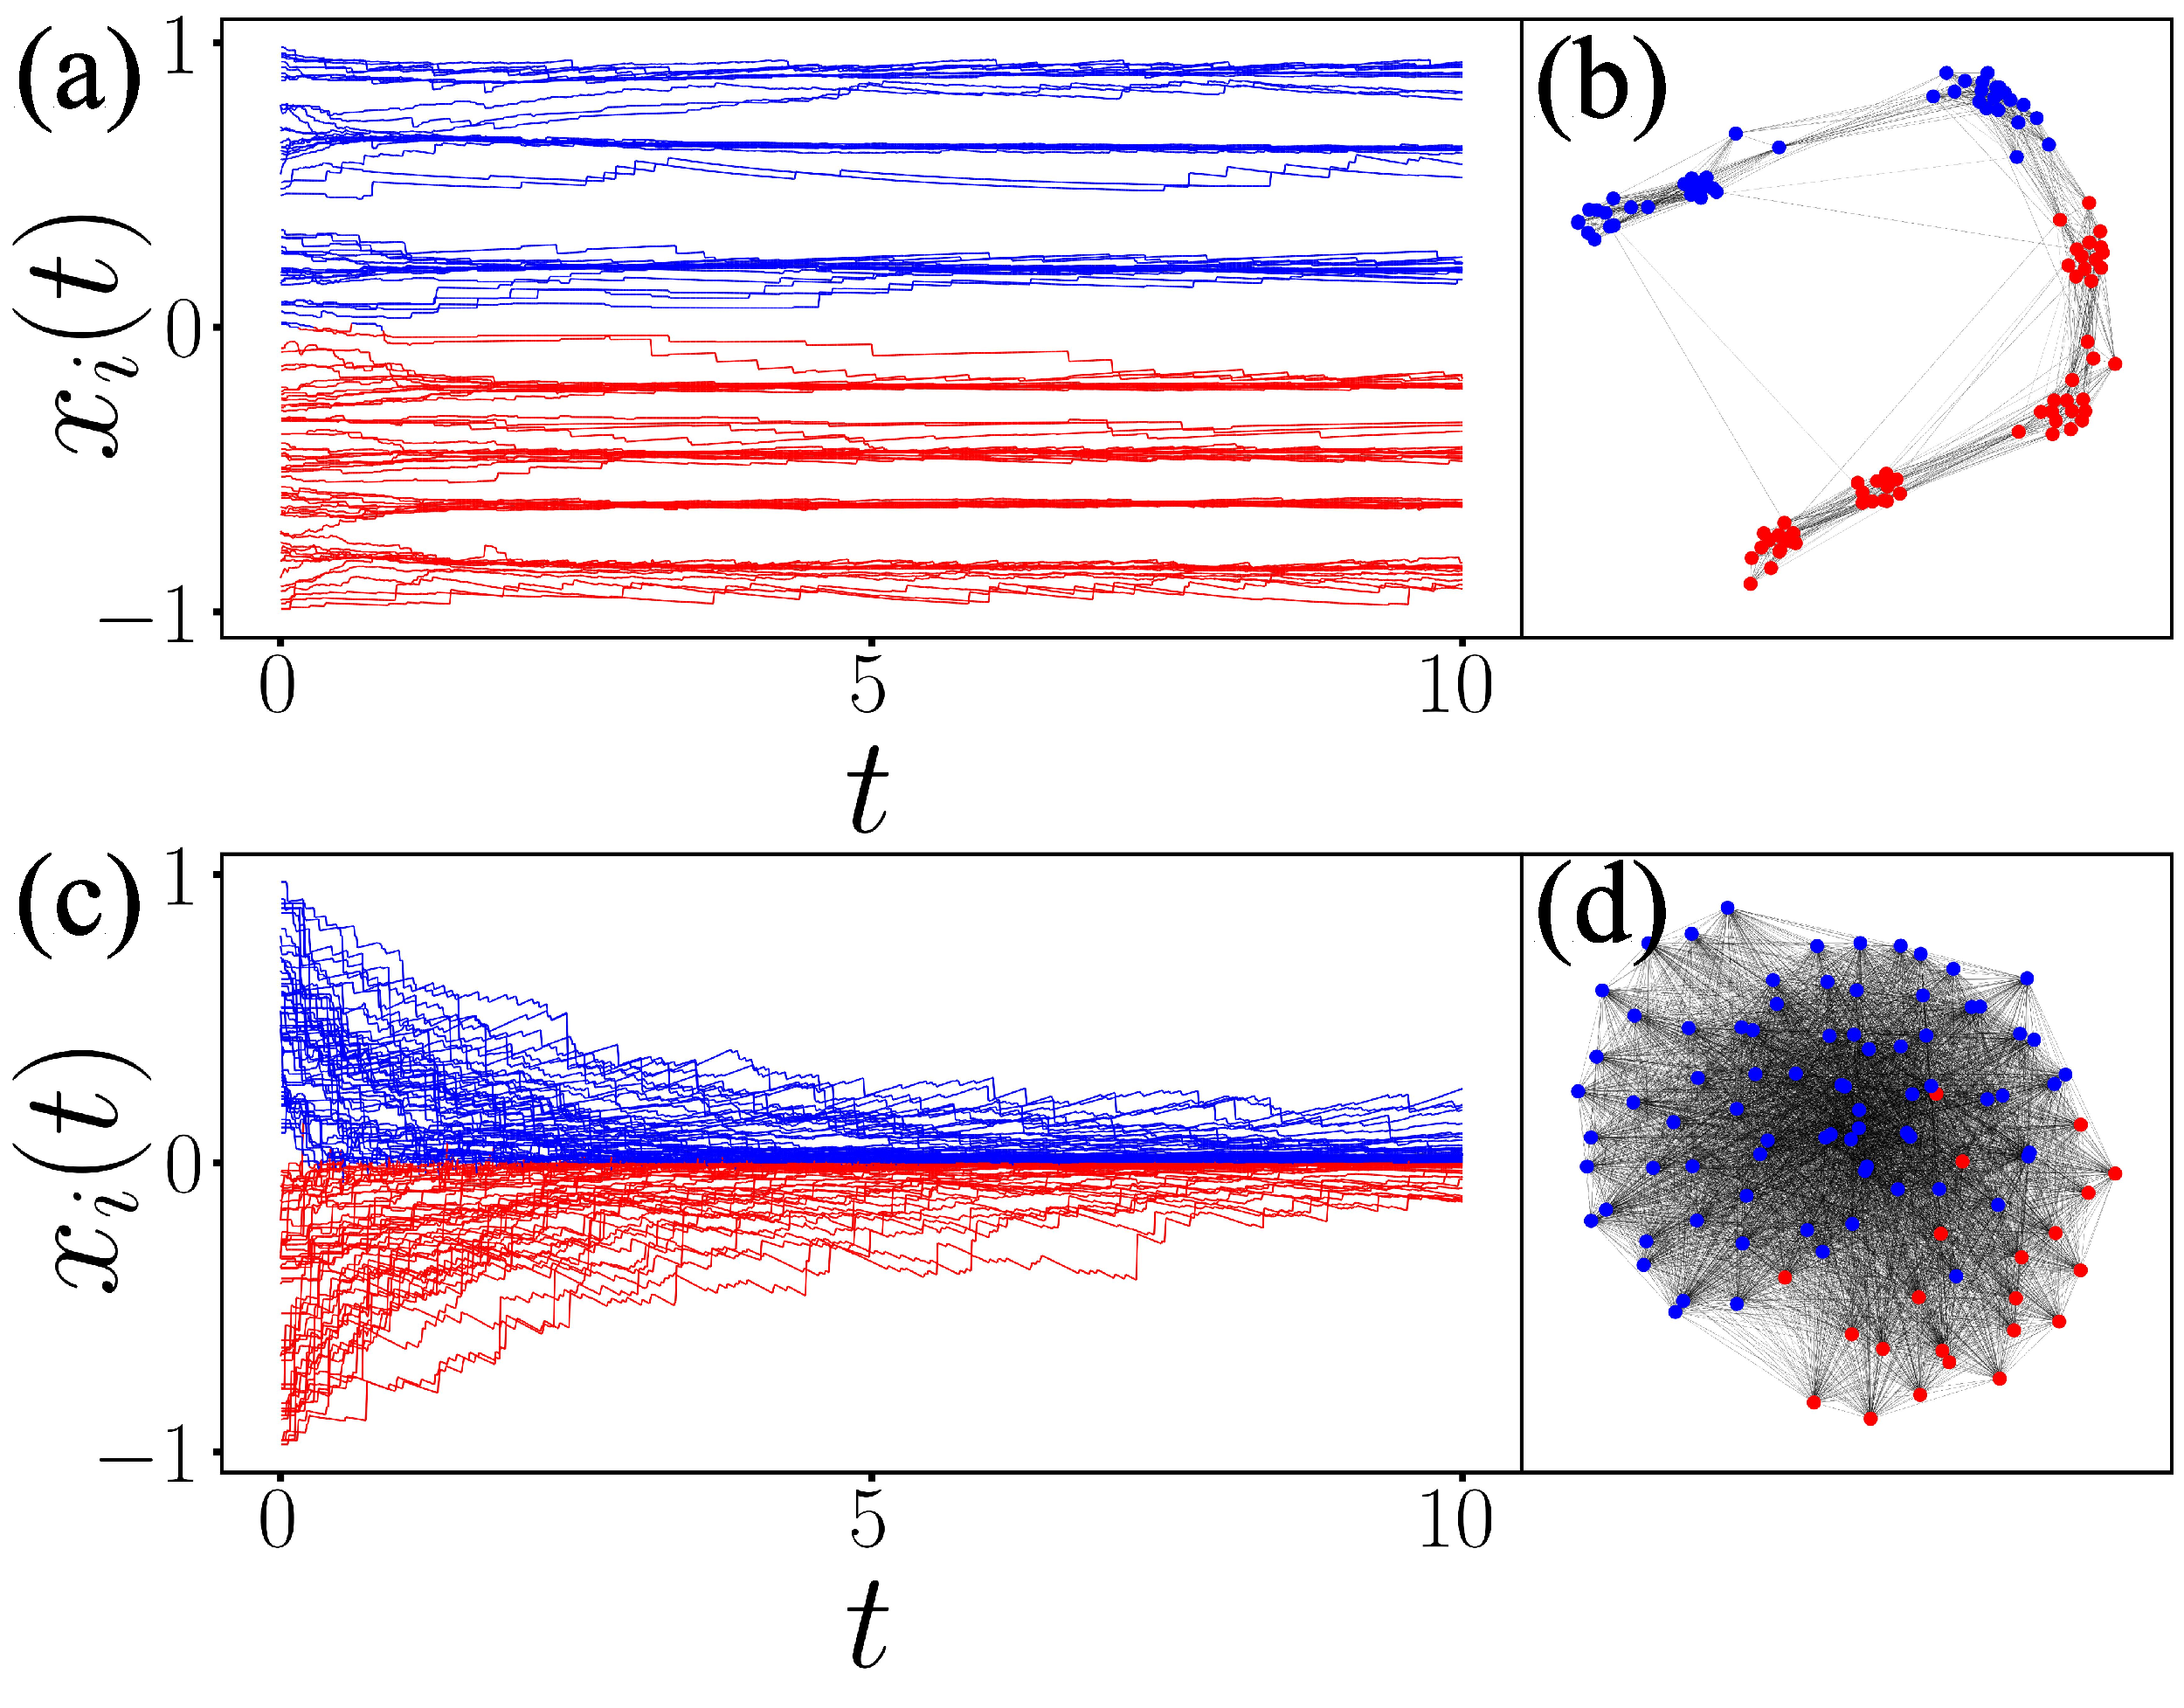
\includegraphics[width=0.8\columnwidth]{chapters/chapter2/new_model.pdf}
    \caption{Demonstration of the random nudge effectiveness in an alternative opinion dynamics model (Equation~\eqref{new_model.eq}). \textbf{(a)} Without nudge: Opinion trajectories display multiple stable clusters, showing the formation of several distinct echo chambers. \textbf{(b)} The corresponding interaction network shows clear community structure with limited cross-group connections. \textbf{(c)} With a small nudge ($p=0.002$): Opinion trajectories converge toward moderate values, showing successful depolarization. \textbf{(d)} The resulting interaction network becomes well-connected without distinct communities. This cross-model validation confirms that the random nudge strategy represents a robust intervention principle applicable across different mathematical frameworks of opinion dynamics.}
    \label{fig:new_model}
\end{figure}
\section{Discussion and Implications}
The widespread use of the internet, and consequently, social media platforms, have drastically altered the way humans consume and interact with information. Polarization and the formation of echo chambers have been shown to negatively impact constructive discussions and debates -- two fundamental pillars of a healthy democracy. Building on the recent advances in the modeling of opinion dynamics in social networks, in this work, we study the possibility of depolarizing a population using a stochastic nudge. The implications of our findings extend beyond digital platforms to broader questions about how collective opinions shape societal outcomes and decision-making processes.
\subsection{Implications for Digital Platform Design}
Our results suggest that a small number of randomized interactions, which are other dominated by homophily-driven mechanisms, can lead to a significant reduction in polarization. This reduction was quantitatively captured by three different measures of polarization. While we show that minimal nudges can burst echo chambers and lead to socially desirable distributions of opinions, increasing the strength of this nudge can result in radicalization. Given this sensitivity on the nudge strength, we show that a possible resolution is obtained if, instead of nudging each agent, only a fraction $f$ of the agents are nudged. We highlight that this interplay of the nudge strength $p$ and the fraction $f$ of nudged individuals leads to an interesting optimization problem. This optimization can help inform the fraction of individuals to be nudged for a fixed nudge strength for optimal depolarization.
\subsection{Ethical Considerations and Implementation Challenges}
We believe that the strongest case for the application of such randomized nudges can be made to recommendation systems. While ubiquitous, recommender algorithms are optimized for increasing engagement \cite{recommender-systems-and-their-ethical-challenges}, which we now know can come at the cost of creating echo chambers \cite{echo-chambers-in-collaborative-filtering-based-recommendation-systems}, increase in the representation of extreme ideologies \cite{recommender-systems-and-the-amplification-of-extremist-content}, and even the tampering of users' preferences \cite{user-tampering}. In such settings, the randomized nudges can be potentially operationalized as the poisoning of a viewer's watch history with a limited amount of random content, uncorrelated with the viewer's preferences \cite{youtube-audit}. While there are several ethical and legal considerations that must be accounted for before implementing any such interventions, it certainly opens up several interesting avenues for future research to build on. Non-invasive interventions may be important to reduce the detrimental effects of polarization. However, an important first step is to build reliable tools to quantify polarization from data \cite{hohmann2023quantifying}, which in itself constitutes an intriguing direction for future research.
\subsection{Broader Implications for Collective Decision-Making}
The random nudge offers a promising, algorithmically implementable strategy for addressing polarization at the individual level. However, this raises important questions about how individual-level interventions might affect collective decision-making processes. The statistical principles underlying opinion formation and the emergence of consensus or polarization may manifest across different scales of human organization. Understanding these connections becomes particularly relevant when considering how societies make collective choices and how the quality of public discourse influences the outcomes of democratic processes. These insights motivate further investigation into the statistical patterns that govern competitive dynamics in various forms of collective decision-making. 

In the next chapter, we will shift our focus from opinion dynamics to electoral systems, examining empirical data from elections across different countries. While not directly employing the opinion models developed here, the underlying theme of how individual choices aggregate into collective outcomes remains central. By analyzing the statistical patterns in election margin distributions, we will uncover universal properties that emerge across diverse electoral systems. These patterns provide a different but complementary perspective on how collective decision-making processes operate at scale, offering insights into the robustness and predictability of democratic institutions regardless of their specific implementation details. 